\begin{abstract}
   En este laboratorio se desarrolló un cruce de semáforo simplificado, conformado por un par de semáforos peatonales y uno vehicular, como se puede observar en la figura \ref{cruce_semaforos}. Dicho sistema debía replicar el comportamiento mostrado en la figura \ref{diagrama_temporizacion} para validar su funcionamiento. Para ello se implementó una máquina de estados a través de un microcontrolador ATtiny4313. Dicha máquina se diseñó con 4 entradas, conformadas por 2 pulsadores y 2 temporizadores. Además cuenta con 4 salidas que representan las luces de los semáforos, y posee un total de 5 estados. Por lo tanto, la máquina requiere únicamente de 1 bit de entrada, ya que los pulsadores están conectados en paralelo como entradas externas del sistema. Añadido a esto, la máquina necesita 3 bits para disponer de 5 combinaciones distintas que identifiquen cada estado. 
   
   \vspace{0.25cm}
   
   Por otro lado, el circuito diseñado para este laboratorio tiene una serie de leds que representan las luces de los semáforos, cada uno acompañado por una resistencia de protección. El circuito también cuenta con un filtro pasivo hecho con una resistencia y un capacitor. Dicho filtro se agregó con el fin de eliminar el factor del ``bouncing'' de los pulsadores.
\end{abstract}

Link del Proyecto: \faGithub   \hspace{0.5mm}\url{https://github.com/Jams1001/IE0624/tree/main/L2} 

\texttt{ID del último commit hecho:\href{https://github.com/Jams1001/IE0624/commit/e99bf4f449cf0c5db9444f61fae2838c64a5bf5a}{e99bf4f449cf0c5db9444f61fae2838c64a5bf5a}}
%\keywords{FEM}

\vspace{0.2cm}

\begin{figure}[H]
    \centering
    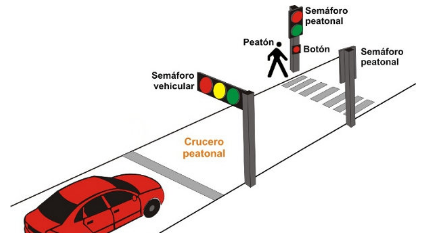
\includegraphics[width=0.575\textwidth]{images/cruce_semaforos.png}
    \caption{Cruce de semáforos simplificado}
    \label{cruce_semaforos}
\end{figure}

\begin{figure}[H]
    \centering
    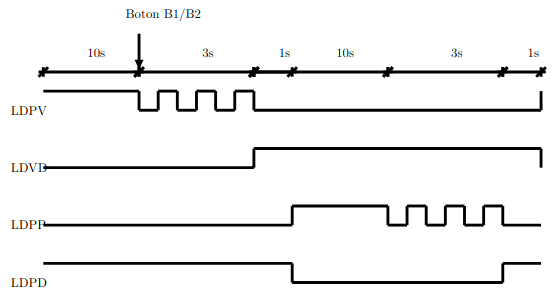
\includegraphics[width=0.65\textwidth]{images/diagrama_temporizacion.png}
    \caption{Diagrama de temporización del cruce de semáforos}
    \label{diagrama_temporizacion}
\end{figure}